\documentclass[12pt]{article}
\usepackage{fontspec}
\usepackage{fullpage}
\usepackage{hyperref}
\hypersetup{bookmarks=true,colorlinks=true,linkcolor=red,citecolor=blue,filecolor=magenta,urlcolor=cyan}
\usepackage{amsmath}
\usepackage{amssymb}
\usepackage{mathtools}
\usepackage{unicode-math}
\usepackage{tabu}
\usepackage{longtable}
\usepackage{booktabs}
\usepackage{caption}
\usepackage{graphics}
\usepackage{enumitem}
\usepackage{filecontents}
\usepackage[backend=bibtex]{biblatex}
\usepackage{url}
\newlist{symbDescription}{description}{1}
\setlist[symbDescription]{noitemsep, topsep=0pt, parsep=0pt, partopsep=0pt}
\setmathfont{Latin Modern Math}
\global\tabulinesep=1mm
\newcounter{assumpnum}
\newcommand{\atheassumpnum}{A\theassumpnum}
\bibliography{bibfile}
\title{Software Requirements Specification for Slope Stability Analysis}
\author{Henry Frankis}
\begin{document}
\maketitle
\tableofcontents
\newpage
\section{Reference Material}
\label{Sec:RefMat}
This section records information for easy reference.
\subsection{Table of Units}
\label{Sec:ToU}
The unit system used throughout is SI (Système International d'Unités). In addition to the basic units, several derived units are also used. For each unit, the table lists the symbol, a description and the SI name.
\begin{longtable*}{l l}
\toprule
Symbol & Description
\\
\midrule
${}^{\circ}$ & angle (degree)
\\
m & length (metre)
\\
N & force (newton)
\\
Pa & pressure (pascal)
\\
\bottomrule
\label{Table:ToU}
\end{longtable*}
\subsection{Table of Symbols}
\label{Sec:ToS}
The table that follows summarizes the symbols used in this document along with their units. Throughout the document, values with a subscript $i$ implies that the value will be taken at and analyzed at a slice or slice interface composing the total slip mass.
\begin{longtabu}{l X[l] l}
\toprule
Symbol & Description & Units
\\
\midrule
$\{{x_{cs}}{,y_{cs}}\}$ & The Set of X and Y Coordinates: describe the vertices of the critical slip surface & m
\\
$(x,y)$ & Cartesian Position Coordinates: y is considered parallel to the direction of the force of gravity and x is considered perpendicular to y & m
\\
$b$ & Base Width of a Slice: in the x-ordinate direction only for slice index i & m
\\
${C1_{i}}$ & Interslice Normal Force Function: the normal force at the interslice interface for slice i & Nm
\\
${C2_{i}}$ & Interslice Shear Force Function: the shear force at the interslice interface for slice i & Nm
\\
$c'$ & Effective Cohesion: internal pressure that sticks particles of soil together & Pa
\\
$f$ & Scaling Function: magnitude of interslice forces as a function of the x coordinatefor interslice index i; can be constant or a half-sine & --
\\
${F_{x}}$ & X-Component of the Net Force:  & N
\\
${F_{y}}$ & Y-Component of the Net Force:  & N
\\
$FS$ & Factor of Safety: The global stability of a surface in a slope & --
\\
${FS_{min}}$ & Minimum Factor of Safety: The minimum factor of safety & --
\\
$G$ & Interslice Normal Force: exerted between adjacent slices for interslice index i & N
\\
$H$ & Interslice Water Force: exerted in the x-ordinate direction between adjacent slices for interslice index i & N
\\
$h$ & Midpoint Height: distance from the slip base to the slope surface in a vertical line from the midpoint of the slice for slice index i & m
\\
$ΔH$ & Difference Between Interslice Forces: exerted in the x-ordinate direction between adjacent slices for interslice index i & N
\\
$i$ & Index: used to show a quantity applies to only one slice & --
\\
${K_{c}}$ & Earthquake Load Factor: proportionality factor of force that weight pushes outwards; caused by seismic earth movements & --
\\
$M$ & Moment: a measure of the tendency of a body to rotate about a specific point or axis & Nm
\\
$N$ & Normal Force: total reactive force for a soil surface subject to a body resting on it & N
\\
$n$ & Number of Slices: the slip mass has been divided into & --
\\
$N'$ & Effective Normal Force: for a soil surface, subtracting pore water reactive force from total reactive force & N
\\
$P$ & Resistive Shear Force: Mohr Coulomb frictional force that describes the limit of mobilized shear force the slice i can withstand before failure & N
\\
$Q$ & Imposed Surface Load: a downward force acting into the surface from midpoint of slice i & N
\\
$R$ & Resistive Shear Force: without the influence of interslice forces for slice index i & N
\\
$S$ & Mobilized Shear Force: for slice index i & N
\\
$SpencerFixme1Please$ & Fixme: What is this value? & --
\\
$SpencerFixme2Please$ & Fixme: What is this value? & --
\\
$T$ & Mobilized Shear Force: without the influence of interslice forces for slice index i & N
\\
$u$ & Local Index: used as a bound variable index in calculations & --
\\
${U_{b}}$ & Base Hydrostatic Force: from water pressure within the slice for slice index i & N
\\
${U_{t}}$ & Surface Hydrostatic Force: from water pressure acting into the slice from standing water on the slope surface for slice index i & N
\\
$v$ & Local Index: used as a bound variable index in calculations & --
\\
$W$ & Weight: downward force caused by gravity on slice i & N
\\
$X$ & Interslice Shear Force: exerted between adjacent slices for interslice index i & N
\\
$x$ & X Ordinate: refers to either slice i midpoint, or slice interface i & m
\\
${x_{slip}}$ & X Ordinate: distance of the slip surface at i, refers to either slice i midpoint, or slice interface i & m
\\
${x_{us}}$ & X Ordinate: distance of the edge of the slope at i, refers to either slice i midpoint, or slice interface i & m
\\
${y_{slip}}$ & Y Ordinate: height of the slip surface at i, refers to either slice i midpoint, or slice interface i & m
\\
${y_{us}}$ & Y Ordinate: height of the top of the slope at i, refers to either slice i midpoint, or slice interface i & m
\\
${y_{wt}}$ & Y Ordinate: height of the water table at i, refers to either slice i midpoint, or slice interface i & m
\\
$z$ & Center of Slice Height: the distance from the lowest part of the slice to the height of the centers of slice & m
\\
$α$ & Angle: base of the mass relative to the horizontal for slice index i & ${}^{\circ}$
\\
$β$ & Angle: surface of the mass relative to the horizontal for slice index i & ${}^{\circ}$
\\
$γ$ & Dry Unit Weight: The weight of a dry soil/ground layer divided by the volume of the layer. & $\frac{\text{N}}{\text{m}^{3}}$
\\
${γ_{Sat}}$ & Saturated Unit Weight: The weight of saturated soil/ground layer divided by the volume of the layer. & $\frac{\text{N}}{\text{m}^{3}}$
\\
${γ_{w}}$ & Unit Weight of Water: The weight of one cubic meter of water. & $\frac{\text{N}}{\text{m}^{3}}$
\\
$λ$ & Interslice Normal/shear Force Ratio: applied to all interslices & --
\\
$μ$ & Pore Pressure: from water within the soil & Pa
\\
$σ$ & Normal Stress: The stress exerted perpendicular to the plane of the object & Pa
\\
$τ$ & Resistive Shear Stress: acting on the base of a slice & Pa
\\
$Υ$ & Function: generic minimization function or algorithm & --
\\
$Φ$ & Constant: converts resistive shear without the influence of interslice forces, to a calculation considering the interslice forces & N
\\
$φ'$ & Effective Angle of Friction: The angle of inclination with respect to the horizontal axis of the Mohr-Coulomb shear resistance line & ${}^{\circ}$
\\
$Ψ$ & Constant: converts mobile shear without the influence of interslice forces, to a calculation considering the interslice forces & N
\\
$ω$ & Angle: of imposed surface load acting into the surface relative to the vertical for slice index i & ${}^{\circ}$
\\
${ℓ_{b}}$ & Total Base Length of a Slice: for slice index i & m
\\
${ℓ_{s}}$ & Length of an Interslice Surface: from slip base to slope surface in a vertical line from an interslice vertex for interslice index i & m
\\
\bottomrule
\label{Table:ToS}
\end{longtabu}
\subsection{Abbreviations and Acronyms}
\label{Sec:TAbbAcc}
\begin{longtable*}{l l}
\toprule
Abbreviation & Full Form
\\
\midrule
A & Assumption
\\
DD & Data Definition
\\
GD & General Definition
\\
GS & Goal Statement
\\
IM & Instance Model
\\
LC & Likely Change
\\
PS & Physical System Description
\\
R & Requirement
\\
SRS & Software Requirements Specification
\\
SSA & Slope Stability Analysis
\\
T & Theoretical Model
\\
UC & Unlikely Change
\\
Uncert. & Typical Uncertainty
\\
\bottomrule
\label{Table:TAbbAcc}
\end{longtable*}
\section{Introduction}
\label{Sec:Intro}
A slope of geological mass, composed of soil and rock, is subject to the influence of gravity on the mass. For an unstable slope this can cause instability in the form of soil/rock movement. The effects of soil/rock movement can range from inconvenient to seriously hazardous, resulting in signifcant life and economic losses. Slope stability is of interest both when analyzing natural slopes, and when designing an excavated slope. Slope stability analysis is the assessment of the safety of a slope, identifying the surface most likely to experience slip and an index of its relative stability known as the factor of safety.
The following section provides an overview of the Software Requirements Specification (SRS) for a slope stability analysis problem. The developed program will be referred to as the Slope Stability Analysis (SSA) program. This section explains the purpose of this document, the scope of the system, the organization of the document, and the characteristics of the intended reader.
\subsection{Purpose of Document}
\label{Sec:DocPurpose}
The SSA program determines the critical slip surface, and its respective factor of safety as a method of assessing the stability of a slope design. The program is intended to be used as an educational tool for introducing slope stability issues, and will facilitate the analysis and design of a safe slope.
This document will be used as a starting point for subsequent development phases, including writing the design specification and the software verification and validation plan. The design document will show how the requirements are to be realized, including decisions on the numerical algorithms and programming environment. The verification and validation plan will show the steps that will be used to increase confidence in the software documentation and the implementation. Although the SRS fits in a series of documents that follow the so-called waterfall model, the actual development process is not constrained in any way. Even when the waterfall model is not followed, as Parnas and Clements point out \cite{parnasClements1986}, the most logical way to present the documentation is still to ``fake'' a rational design process.
\subsection{Scope of Requirements}
\label{Sec:ReqsScope}
The scope of the requirements includes stability analysis of a 2 dimensional slope, composed of homogeneous soil layers. Given the appropriate inputs, SSA identifies the most likely failure surface within the possible input range, and finds the factor of safety for the slope.
\subsection{Characteristics of Intended Reader}
\label{Sec:ReaderChars}
Reviewers of this documentation should have a strong knowledge in solid mechanics. The reviewers should also have an understanding of undergraduate level 4 physics. The users of SSA can have a lower level of expertise, as explained in \hyperref[Sec:UserChars]{Section: User Characteristics}.
\subsection{Organization of Document}
\label{Sec:DocOrg}
The organization of this document follows the template for an SRS for scientific computing software proposed by Koothoor as well as Smith and Lai. The presentation follows the standard pattern of presenting goals, theories, definitions, and assumptions. For readers that would like a more bottom up approach, they can start reading the instance models in \hyperref[Sec:IMs]{Instance Models} and trace back to find any additional information they require.
The goal statements are refined to the theoretical models, and the theoretical models to the instance models. The instance models provide the set of algebraic equations that must be solved iteratively to perform a Morgenstern Price Analysis.
\section{General System Description}
\label{Sec:GenSysDesc}
This section provides general information about the system including identifying the interfaces between the system and its environment (system context), describing the user characteristics and listing the system constraints.
\subsection{System Context}
\label{Sec:SysContext}
\hyperref[Figure:sysCtxDiag]{Fig:sysCtxDiag} shows the system context. A circle represents an external entity outside the software, the user in this case. A rectangle represents the software system itself (SSP). Arrows are used to show the data flow between the system and its environment.
\begin{figure}
\begin{center}
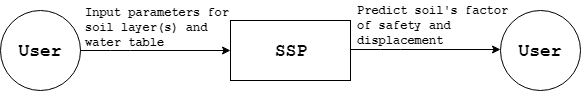
\includegraphics[width=\textwidth]{../../../datafiles/SSP/SystemContextFigure.png}
\caption{System Context}
\label{Figure:sysCtxDiag}
\end{center}
\end{figure}
The interaction between the product and the user is through a user interface. The responsibilities of the user and the system are as follows:
\begin{itemize}
\item{User Responsibilities}
\begin{itemize}
\item{Provide the input data related to the soil layer(s) and water table (if applicable), ensuring no errors in the data entry}
\item{Ensure that consistent units are used for input variables}
\item{Ensure required software assumptions (\hyperref[Sec:Assumps]{Section: Assumptions}) are appropriate for any particular problem input to the software}
\end{itemize}
\item{SSP Responsibilities}
\begin{itemize}
\item{Detect data type mismatch, such as a string of characters  input instead of a floating point number}
\item{Determine if the inputs satisfy the required physical and software constraints}
\item{Identify the most likely failure surface within the possible input range}
\item{Find the factor of safety for the slope}
\end{itemize}
\end{itemize}
\subsection{User Characteristics}
\label{Sec:UserChars}
The end user of SSA should have an understanding of undergraduate Level 1 Calculus and Physics, and be familiar with soil and material properties.
\subsection{System Constraints}
\label{Sec:SysConstraints}
There are no system constraints.
\section{Specific System Description}
\label{Sec:SpecSystDesc}
This section first presents the problem description, which gives a high-level view of the problem to be solved. This is followed by the solution characteristics specification, which presents the assumptions, theories, and definitions that are used.
\subsection{Problem Description}
\label{Sec:ProbDesc}
SSA is a computer program developed to evaluate the factor of safety of a slope's slip surface and identify the critical slip surface of the slope.
\subsubsection{Terminology and Definitions}
\label{Sec:TermDefs}
This subsection provides a list of terms that are used in the subsequent sections and their meaning, with the purpose of reducing ambiguity and making it easier to correctly understand the requirements.
\begin{itemize}
\item[Factor of Safety:]The global stability of a surface in a slope
\item[Critical Slip Surface:]Slip surface of the slope that has the lowest global factor of safety, and therefore most likely to experience failure.
\item[Stress:]Forces that are exerted between planes internal to a larger body subject to external loading.
\item[Strain:]Stress forces that result in deformation of the body/plane.
\item[Normal Force:]A force applied perpendicular to the plane of the material.
\item[Shear Force:]A force applied parallel to the plane of the material.
\item[Plane Strain:]The resultant stresses in one of the directions of a 3 dimensional material can be approximated as 0. Results when the length of one dimension of the body dominates the others. Stresses in the dominant dimensions direction are the ones that can be approximated as 0.
\end{itemize}
\subsubsection{Physical System Description}
\label{Sec:PhysSyst}
Analysis of the slope is performed by looking at properties of the slope as a series of slice elements. Some properties are interslice properties, and some are slice or slice base properties. The index convention for referencing which interslice or slice is being used is shown in \hyperref[Figure:IndexConvention]{Fig:IndexConvention}.
\begin{itemize}
\item[PS1:]Interslice properties convention is noted by j. The end interslice properties are usually not of interest, therefore use the interslice properties from $1\leq{}i\leq{}n-1$.
\item[PS2:]Slice properties convention is noted by $i$.
\end{itemize}
A free body diagram of the forces acting on the slice is displayed in \hyperref[Figure:ForceDiagram]{Fig:ForceDiagram}.
\begin{figure}
\begin{center}
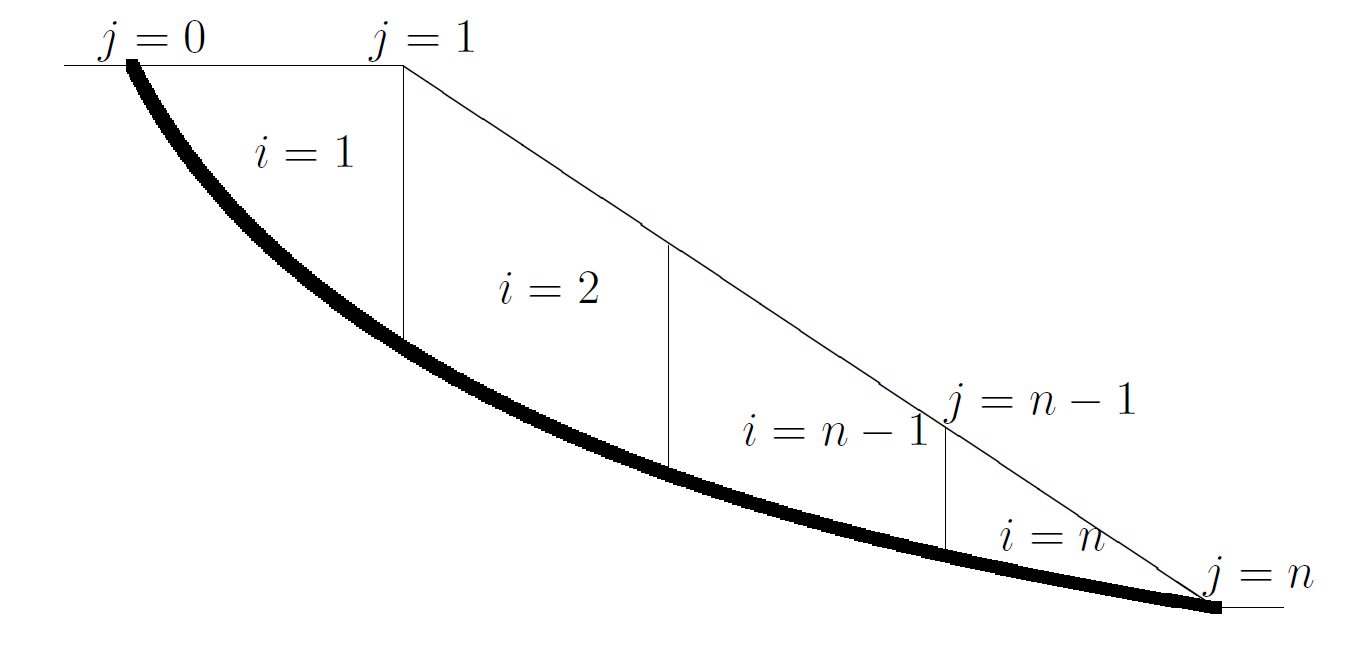
\includegraphics[width=\textwidth]{../../../datafiles/SSP/IndexConvention.png}
\caption{Index convention for numbering slice and interslice force variables}
\label{Figure:IndexConvention}
\end{center}
\end{figure}
\begin{figure}
\begin{center}
\includegraphics[width=\textwidth]{../../../datafiles/SSP/ForceDiagram.png}
\caption{Forces acting on a slice}
\label{Figure:ForceDiagram}
\end{center}
\end{figure}
\subsubsection{Goal Statements}
\label{Sec:GoalStmt}
Given the geometry of the water table, the geometry of the layers composing the plane of a slope, and the material properties of the layers, the goal statements are:
\begin{itemize}
\item[GS1:]Evaluate the factor of safety along a given slip surface.
\item[GS2:]Identify the critical slip surface for the slope, with the lowest factor of safety.
\end{itemize}
\subsection{Solution Characteristics Specification}
\label{Sec:SolCharSpec}
The instance models that govern SSA are presented in \hyperref[Sec:IMs]{Section: Instance Models}. The information to understand the meaning of the instance models and their derivation is also presented, so that the instance models can be verified.
\subsubsection{Assumptions}
\label{Sec:Assumps}
This section simplifies the original problem and helps in developing the theoretical model by filling in the missing information for the physical system. The numbers given in the square brackets refer to the Theoretical Models {[}\hyperref[Sec:TMs]{Section: Theoretical Models}{]}, General Definitions {[}\hyperref[Sec:GDs]{Section: General Definitions}{]}, Data Definitions {[}\hyperref[Sec:DDs]{Section: Data Definitions}{]}, Instance Models {[}\hyperref[Sec:IMs]{Section: Instance Models}{]}, Likely Changes {[}\hyperref[Sec:LCs]{Section: Likely Changes}{]}, or Unlikely Changes {[}\hyperref[Sec:UCs]{Section: Unlikely Changes}{]}, in which the respective assumption is used.
\begin{description}
\item[\refstepcounter{assumpnum}\atheassumpnum\label{A:Slip-Surface-Concave}:]The slip surface is concave with respect to the slope surface. The $(x,y)$ coordinates of the failure surface follow a monotonic function.
\end{description}
\begin{description}
\item[\refstepcounter{assumpnum}\atheassumpnum\label{A:Factor-of-Safety}:]The factor of safety is assumed to be constant across a whole slip surface. \hyperref[GD:mobShr]{GD: mobShr} \hyperref[IM:intsliceFs]{IM: intsliceFs} \hyperref[IM:fctSfty]{IM: fctSfty}.
\end{description}
\begin{description}
\item[\refstepcounter{assumpnum}\atheassumpnum\label{A:Soil-Layer-Homogeneous}:]The different layers of the soil are homogeneous, with consistent soil properties throughout. \hyperref[GD:resShr]{GD: resShr} \hyperref[GD:mobShr]{GD: mobShr} \hyperref[LC_inhomogeneous]{LC: Calculate-Inhomogeneous-Soil-Layers}.
\end{description}
\begin{description}
\item[\refstepcounter{assumpnum}\atheassumpnum\label{A:Soil-Properties}:]The soil properties are independent of dry or saturated conditions, with the exception of unit weight. \hyperref[GD:resShr]{GD: resShr} \hyperref[GD:mobShr]{GD: mobShr} \hyperref[IM:crtSlpId]{IM: crtSlpId}.
\end{description}
\begin{description}
\item[\refstepcounter{assumpnum}\atheassumpnum\label{A:Soil-Layers-Isotropic}:]Soil layers are treated as if they have isotropic properties. \hyperref[GD:resShr]{GD: resShr} \hyperref[GD:mobShr]{GD: mobShr} \hyperref[UC_normshearlinear]{UC: Normal-And-Shear-Linear-Only}.
\end{description}
\begin{description}
\item[\refstepcounter{assumpnum}\atheassumpnum\label{A:Interslice-Norm-Shear-Forces-Linear}:]Interslice normal and shear forces have a linear relationship, proportional to a constant ($λ$) and an interslice force function ($f$) depending on x position. \hyperref[IM:nrmShrFor]{IM: nrmShrFor} \hyperref[GD:normShrR]{GD: normShrR} \hyperref[GD:momentEql]{GD: momentEql} \hyperref[IM:intsliceFs]{IM: intsliceFs} \hyperref[IM:fctSfty]{IM: fctSfty} \hyperref[UC_normshearlinear]{UC: Normal-And-Shear-Linear-Only}.
\end{description}
\begin{description}
\item[\refstepcounter{assumpnum}\atheassumpnum\label{A:Plane-Strain-Conditions}:]The slope and slip surface extends far into and out of the geometry (z coordinate). This implies plane strain conditions, making 2D analysis appropriate.
\end{description}
\begin{description}
\item[\refstepcounter{assumpnum}\atheassumpnum\label{A:Effective-Norm-Stress-Large}:]The effective normal stress is large enough that the resistive shear to effective normal stress relationship can be approximated as a linear relationship. \hyperref[T:equilibrium]{TM: equilibrium} \hyperref[UC_2donly]{UC: 2D-Analysis-Only}.
\end{description}
\begin{description}
\item[\refstepcounter{assumpnum}\atheassumpnum\label{A:Surface-Base-Slice-between-Interslice-Straight-Lines}:]The surface and base of a slice between interslice nodes are approximated as straight lines. \hyperref[T:mcShrStrgth]{TM: mcShrStrgth} \hyperref[DD:lengthLs]{DD: lengthLs} \hyperref[DD:lengthLb]{DD: lengthLb} \hyperref[DD:angleB]{DD: angleB} \hyperref[DD:angleA]{DD: angleA} \hyperref[DD:surfWtrF]{DD: surfWtrF} \hyperref[DD:baseWtrF]{DD: baseWtrF}.
\end{description}
\begin{description}
\item[\refstepcounter{assumpnum}\atheassumpnum\label{A:Seismic-Force}:]There is no seismic force acting on the slope. \hyperref[IM:nrmShrFor]{IM: nrmShrFor} \hyperref[IM:intsliceFs]{IM: intsliceFs} \hyperref[IM:fctSfty]{IM: fctSfty}.
\end{description}
\begin{description}
\item[\refstepcounter{assumpnum}\atheassumpnum\label{A:Surface-Load}:]There is no imposed surface, load and therefore no external force, acting on the slope. \hyperref[IM:nrmShrFor]{IM: nrmShrFor} \hyperref[IM:intsliceFs]{IM: intsliceFs} \hyperref[IM:fctSfty]{IM: fctSfty}.
\end{description}
\subsubsection{Theoretical Models}
\label{Sec:TMs}
This section focuses on the general equations and laws that SSA is based on.
~\newline
\noindent \begin{minipage}{\textwidth}
\begin{tabular}{p{0.2\textwidth} p{0.73\textwidth}}
\toprule \textbf{Refname} & \textbf{T:factOfSafety}
\phantomsection 
\label{T:factOfSafety}
\\ \midrule \\
Label & Factor of safety
\\ \midrule \\
Equation & \begin{dmath}
           FS=\frac{P}{S}
           \end{dmath}
\\ \midrule \\
Description & \begin{symbDescription}
              \item{$FS$ is the factor of safety (Unitless)}
              \item{$P$ is the resistive shear force (N)}
              \item{$S$ is the mobilized shear force (N)}
              \end{symbDescription}
\\ \midrule \\
Notes & The stability metric of the slope, known as the factor of safety ($FS$), is determined by the ratio of the shear force at the base of the slope ($S$), and the resistive shear ($P$).
\\ \midrule \\
Source & \cite{fredlund1977}
\\ \midrule \\
RefBy & \hyperref[GD:mobShr]{GD: mobShr}.
\\ \bottomrule \end{tabular}
\end{minipage}\\
~\newline
\noindent \begin{minipage}{\textwidth}
\begin{tabular}{p{0.2\textwidth} p{0.73\textwidth}}
\toprule \textbf{Refname} & \textbf{T:equilibrium}
\phantomsection 
\label{T:equilibrium}
\\ \midrule \\
Label & Equilibrium
\\ \midrule \\
Equation & \begin{dmath}
           \displaystyle\sum{{F_{x}}}=\displaystyle\sum{{F_{y}}}=\displaystyle\sum{M}=0
           \end{dmath}
\\ \midrule \\
Description & \begin{symbDescription}
              \item{${F_{x}}$ is the x-component of the net force (N)}
              \item{${F_{y}}$ is the y-component of the net force (N)}
              \item{$M$ is the moment (Nm)}
              \end{symbDescription}
\\ \midrule \\
Notes & For a body in static equilibrium, the net forces and net moments acting on the body will cancel out. Assuming a 2D problem (\hyperref[A:Effective-Norm-Stress-Large]{A: Effective-Norm-Stress-Large}) the x-component of the net force ${F_{x}}$ and y-component of the net force ${F_{y}}$ will be equal to $0$. All forces and their distance from the chosen point of rotation will create a net moment equal to $0$.
\\ \midrule \\
Source & \cite{fredlund1977}
\\ \midrule \\
RefBy & \hyperref[GD:normForcEq]{GD: normForcEq} \hyperref[GD:momentEql]{GD: momentEql} \hyperref[GD:bsShrFEq]{GD: bsShrFEq}.
\\ \bottomrule \end{tabular}
\end{minipage}\\
~\newline
\noindent \begin{minipage}{\textwidth}
\begin{tabular}{p{0.2\textwidth} p{0.73\textwidth}}
\toprule \textbf{Refname} & \textbf{T:mcShrStrgth}
\phantomsection 
\label{T:mcShrStrgth}
\\ \midrule \\
Label & Mohr-Coulumb shear strength
\\ \midrule \\
Equation & \begin{dmath}
           τ=σ \tan\left(φ'\right)+c'
           \end{dmath}
\\ \midrule \\
Description & \begin{symbDescription}
              \item{$τ$ is the resistive shear stress (Pa)}
              \item{$σ$ is the normal stress (Pa)}
              \item{$φ'$ is the effective angle of friction (${}^{\circ}$)}
              \item{$c'$ is the effective cohesion (Pa)}
              \end{symbDescription}
\\ \midrule \\
Notes & For a soil under stress it will exert a shear resistive strength based on the Coulomb sliding law. The resistive shear is the maximum amount of shear a surface can experience while remaining rigid, analogous to a maximum normal force. In this model the resistive shear stress $τ$ is proportional to the product of the normal stress on the plane $σ$ with it's static friction in the angular form $\tan\left(φ'\right)={U_{t}}$. The $τ$ versus $σ$ relationship is not truly linear, but assuming the effective normal force is strong enough, it can be approximated with a linear fit (\hyperref[A:Surface-Base-Slice-between-Interslice-Straight-Lines]{A: Surface-Base-Slice-between-Interslice-Straight-Lines}) where the cohesion $c'$ represents the $τ$ intercept of the fitted line.
\\ \midrule \\
Source & \cite{fredlund1977}
\\ \midrule \\
RefBy & \hyperref[GD:resShr]{GD: resShr}.
\\ \bottomrule \end{tabular}
\end{minipage}\\
~\newline
\noindent \begin{minipage}{\textwidth}
\begin{tabular}{p{0.2\textwidth} p{0.73\textwidth}}
\toprule \textbf{Refname} & \textbf{T:effStress}
\phantomsection 
\label{T:effStress}
\\ \midrule \\
Label & Effective stress
\\ \midrule \\
Equation & \begin{dmath}
           σ=σ-μ
           \end{dmath}
\\ \midrule \\
Description & \begin{symbDescription}
              \item{$σ$ is the normal stress (Pa)}
              \item{$μ$ is the pore pressure (Pa)}
              \end{symbDescription}
\\ \midrule \\
Notes & $σ$ is the total stress a soil mass needs to maintain itself as a rigid collection of particles. The source of the stress can be provided by the soil skeleton $σ$, or by the pore pressure from water within the soil $μ$. The stress from the soil skeleton is known as the effective stress $σ$ and is the difference between the total stress $σ$ and the pore stress $μ$.
\\ \midrule \\
Source & \cite{fredlund1977}
\\ \midrule \\
RefBy & \hyperref[GD:resShr]{GD: resShr}.
\\ \bottomrule \end{tabular}
\end{minipage}\\
\subsubsection{General Definitions}
\label{Sec:GDs}
This section collects the laws and equations that will be used in deriving the data definitions, which in turn are used to build the instance models.
~\newline
\noindent \begin{minipage}{\textwidth}
\begin{tabular}{p{0.2\textwidth} p{0.73\textwidth}}
\toprule \textbf{Refname} & \textbf{GD:normForcEq}
\phantomsection 
\label{GD:normForcEq}
\\ \midrule \\
Label & Normal force equilibrium
\\ \midrule \\
Equation & \begin{dmath}
           N_{i}=\left(W_{i}-X_{i-1}+X_{i}+{U_{t,i}} \cos\left(β_{i}\right)+Q_{i} \cos\left(ω_{i}\right)\right) \cos\left(α_{i}\right)+\left(-{K_{c}} W_{i}-G_{i}+G_{i-1}-H_{i}+H_{i-1}+{U_{t,i}} \sin\left(β_{i}\right)+Q_{i} \sin\left(ω_{i}\right)\right) \sin\left(α_{i}\right)
           \end{dmath}
\\ \midrule \\
Description & \begin{symbDescription}
              \item{$N$ is the normal force (N)}
              \item{$i$ is the index (Unitless)}
              \item{$W$ is the weight (N)}
              \item{$X$ is the interslice shear force (N)}
              \item{${U_{t}}$ is the surface hydrostatic force (N)}
              \item{$β$ is the angle (${}^{\circ}$)}
              \item{$Q$ is the imposed surface load (N)}
              \item{$ω$ is the angle (${}^{\circ}$)}
              \item{$α$ is the angle (${}^{\circ}$)}
              \item{${K_{c}}$ is the earthquake load factor (Unitless)}
              \item{$G$ is the interslice normal force (N)}
              \item{$H$ is the interslice water force (N)}
              \end{symbDescription}
\\ \midrule \\
Notes & This equation satisfies \hyperref[T:equilibrium]{TM: equilibrium} in the shear direction. Force equilibrium is derived from the free body diagram of \hyperref[Figure:ForceDiagram]{Fig:ForceDiagram} in \hyperref[Sec:PhysSyst]{Section: Physical System Description}.
\\ \midrule \\
Source & \cite{chen2005}
\\ \midrule \\
RefBy & \hyperref[IM:intsliceFs]{IM: intsliceFs}.
\\ \bottomrule \end{tabular}
\end{minipage}\\
~\newline
\noindent \begin{minipage}{\textwidth}
\begin{tabular}{p{0.2\textwidth} p{0.73\textwidth}}
\toprule \textbf{Refname} & \textbf{GD:bsShrFEq}
\phantomsection 
\label{GD:bsShrFEq}
\\ \midrule \\
Label & Base shear force equilibrium
\\ \midrule \\
Equation & \begin{dmath}
           S_{i}=\left(W_{i}-X_{i-1}+X_{i}+{U_{t,i}} \cos\left(β_{i}\right)+Q_{i} \cos\left(ω_{i}\right)\right) \sin\left(α_{i}\right)-\left(-{K_{c}} W_{i}-G_{i}+G_{i-1}-H_{i}+H_{i-1}+{U_{t,i}} \sin\left(β_{i}\right)+Q_{i} \sin\left(ω_{i}\right)\right) \cos\left(α_{i}\right)
           \end{dmath}
\\ \midrule \\
Description & \begin{symbDescription}
              \item{$S$ is the mobilized shear force (N)}
              \item{$i$ is the index (Unitless)}
              \item{$W$ is the weight (N)}
              \item{$X$ is the interslice shear force (N)}
              \item{${U_{t}}$ is the surface hydrostatic force (N)}
              \item{$β$ is the angle (${}^{\circ}$)}
              \item{$Q$ is the imposed surface load (N)}
              \item{$ω$ is the angle (${}^{\circ}$)}
              \item{$α$ is the angle (${}^{\circ}$)}
              \item{${K_{c}}$ is the earthquake load factor (Unitless)}
              \item{$G$ is the interslice normal force (N)}
              \item{$H$ is the interslice water force (N)}
              \end{symbDescription}
\\ \midrule \\
Notes & This equation satisfies \hyperref[T:equilibrium]{TM: equilibrium} in the shear direction. Force equilibrium is derived from the free body diagram of \hyperref[Figure:ForceDiagram]{Fig:ForceDiagram} in \hyperref[Sec:PhysSyst]{Section: Physical System Description}.
\\ \midrule \\
Source & \cite{chen2005}
\\ \midrule \\
RefBy & \hyperref[IM:intsliceFs]{IM: intsliceFs}.
\\ \bottomrule \end{tabular}
\end{minipage}\\
~\newline
\noindent \begin{minipage}{\textwidth}
\begin{tabular}{p{0.2\textwidth} p{0.73\textwidth}}
\toprule \textbf{Refname} & \textbf{GD:resShr}
\phantomsection 
\label{GD:resShr}
\\ \midrule \\
Label & Resistive shear force
\\ \midrule \\
Equation & \begin{dmath}
           P_{i}={N'}_{i} \tan\left({φ'}_{i}\right)+{c'}_{i} b_{i} \sec\left(α_{i}\right)
           \end{dmath}
\\ \midrule \\
Description & \begin{symbDescription}
              \item{$P$ is the resistive shear force (N)}
              \item{$i$ is the index (Unitless)}
              \item{$N'$ is the effective normal force (N)}
              \item{$φ'$ is the effective angle of friction (${}^{\circ}$)}
              \item{$c'$ is the effective cohesion (Pa)}
              \item{$b$ is the base width of a slice (m)}
              \item{$α$ is the angle (${}^{\circ}$)}
              \end{symbDescription}
\\ \midrule \\
Notes & The Mohr-Coulomb resistive shear strength of a slice $τ$ from \hyperref[T:mcShrStrgth]{TM: mcShrStrgth} is multiplied by the area $b \sec\left(α\right)\cdot{}1$ to obtain the resistive shear force $P$. Note the extra $1$ is to represent a unit of width which is multiplied by the total base length of a slice ${ℓ_{b}}$ of the plane where the normal occurs, where ${ℓ_{b}}=b \sec\left(α\right)$ and $b$ is the x width of the base. This accounts for the effective normal force $N'=N-{U_{b}}$ of a soil from \hyperref[T:effStress]{TM: effStress} where the normal stress is multiplied by the same area to obtain the effective normal force $σ b \sec\left(α\right)\cdot{}1=N'$ \hyperref[A:Soil-Layer-Homogeneous]{A: Soil-Layer-Homogeneous} \hyperref[A:Soil-Properties]{A: Soil-Properties} \hyperref[A:Soil-Layers-Isotropic]{A: Soil-Layers-Isotropic}
\\ \midrule \\
Source & \cite{chen2005}
\\ \midrule \\
RefBy & \hyperref[GD:mobShr]{GD: mobShr}.
\\ \bottomrule \end{tabular}
\end{minipage}\\
~\newline
\noindent \begin{minipage}{\textwidth}
\begin{tabular}{p{0.2\textwidth} p{0.73\textwidth}}
\toprule \textbf{Refname} & \textbf{GD:mobShr}
\phantomsection 
\label{GD:mobShr}
\\ \midrule \\
Label & Mobile shear force
\\ \midrule \\
Equation & \begin{dmath}
           S_{i}=\frac{P_{i}}{FS}=\frac{{N'}_{i} \tan\left({φ'}_{i}\right)+{c'}_{i} b_{i} \sec\left(α_{i}\right)}{FS}
           \end{dmath}
\\ \midrule \\
Description & \begin{symbDescription}
              \item{$S$ is the mobilized shear force (N)}
              \item{$i$ is the index (Unitless)}
              \item{$P$ is the resistive shear force (N)}
              \item{$FS$ is the factor of safety (Unitless)}
              \item{$N'$ is the effective normal force (N)}
              \item{$φ'$ is the effective angle of friction (${}^{\circ}$)}
              \item{$c'$ is the effective cohesion (Pa)}
              \item{$b$ is the base width of a slice (m)}
              \item{$α$ is the angle (${}^{\circ}$)}
              \end{symbDescription}
\\ \midrule \\
Notes & From the definition of the factor of safety in \hyperref[T:factOfSafety]{TM: factOfSafety}, and the new definition of $P$, a new relation for the net mobile shear force of the slice $T$ is found as the resistive shear $P$ (\hyperref[GD:resShr]{GD: resShr}) divided by the factor of safety $FS$. \hyperref[A:Factor-of-Safety]{A: Factor-of-Safety} \hyperref[A:Soil-Layer-Homogeneous]{A: Soil-Layer-Homogeneous} \hyperref[A:Soil-Properties]{A: Soil-Properties} \hyperref[A:Soil-Layers-Isotropic]{A: Soil-Layers-Isotropic}
\\ \midrule \\
Source & \cite{chen2005}
\\ \midrule \\
RefBy & \hyperref[IM:intsliceFs]{IM: intsliceFs}.
\\ \bottomrule \end{tabular}
\end{minipage}\\
~\newline
\noindent \begin{minipage}{\textwidth}
\begin{tabular}{p{0.2\textwidth} p{0.73\textwidth}}
\toprule \textbf{Refname} & \textbf{GD:resShearWO}
\phantomsection 
\label{GD:resShearWO}
\\ \midrule \\
Label & Resistive shear force
\\ \midrule \\
Equation & \begin{dmath}
           R=\left(\left(W_{i}+{U_{t,i}} \cos\left(β_{i}\right)+Q_{i} \cos\left(ω_{i}\right)\right) \cos\left(α_{i}\right)+\left(-{K_{c}} W_{i}-{ΔH}_{i}+{U_{t,i}} \sin\left(β_{i}\right)+Q_{i} \sin\left(ω_{i}\right)\right) \sin\left(α_{i}\right)-{U_{b,i}}\right) \tan\left({φ'}_{i}\right)+{c'}_{i} b_{i} \sec\left(α_{i}\right)
           \end{dmath}
\\ \midrule \\
Description & \begin{symbDescription}
              \item{$R$ is the resistive shear force (N)}
              \item{$W$ is the weight (N)}
              \item{$i$ is the index (Unitless)}
              \item{${U_{t}}$ is the surface hydrostatic force (N)}
              \item{$β$ is the angle (${}^{\circ}$)}
              \item{$Q$ is the imposed surface load (N)}
              \item{$ω$ is the angle (${}^{\circ}$)}
              \item{$α$ is the angle (${}^{\circ}$)}
              \item{${K_{c}}$ is the earthquake load factor (Unitless)}
              \item{$ΔH$ is the difference between interslice forces (N)}
              \item{${U_{b}}$ is the base hydrostatic force (N)}
              \item{$φ'$ is the effective angle of friction (${}^{\circ}$)}
              \item{$c'$ is the effective cohesion (Pa)}
              \item{$b$ is the base width of a slice (m)}
              \end{symbDescription}
\\ \midrule \\
Source & \cite{chen2005}
\\ \midrule \\
RefBy & \hyperref[IM:intsliceFs]{IM: intsliceFs} \hyperref[IM:intsliceFs]{IM: intsliceFs}.
\\ \bottomrule \end{tabular}
\end{minipage}\\
~\newline
\noindent \begin{minipage}{\textwidth}
\begin{tabular}{p{0.2\textwidth} p{0.73\textwidth}}
\toprule \textbf{Refname} & \textbf{GD:mobShearWO}
\phantomsection 
\label{GD:mobShearWO}
\\ \midrule \\
Label & Mobilized shear force
\\ \midrule \\
Equation & \begin{dmath}
           T=\left(W_{i}+{U_{t,i}} \cos\left(β_{i}\right)+Q_{i} \cos\left(ω_{i}\right)\right) \sin\left(α_{i}\right)-\left(-{K_{c}} W_{i}-{ΔH}_{i}+{U_{t,i}} \sin\left(β_{i}\right)+Q_{i} \sin\left(ω_{i}\right)\right) \cos\left(α_{i}\right)
           \end{dmath}
\\ \midrule \\
Description & \begin{symbDescription}
              \item{$T$ is the mobilized shear force (N)}
              \item{$W$ is the weight (N)}
              \item{$i$ is the index (Unitless)}
              \item{${U_{t}}$ is the surface hydrostatic force (N)}
              \item{$β$ is the angle (${}^{\circ}$)}
              \item{$Q$ is the imposed surface load (N)}
              \item{$ω$ is the angle (${}^{\circ}$)}
              \item{$α$ is the angle (${}^{\circ}$)}
              \item{${K_{c}}$ is the earthquake load factor (Unitless)}
              \item{$ΔH$ is the difference between interslice forces (N)}
              \end{symbDescription}
\\ \midrule \\
Source & \cite{chen2005}
\\ \midrule \\
RefBy & \hyperref[IM:intsliceFs]{IM: intsliceFs} \hyperref[IM:intsliceFs]{IM: intsliceFs}.
\\ \bottomrule \end{tabular}
\end{minipage}\\
~\newline
\noindent \begin{minipage}{\textwidth}
\begin{tabular}{p{0.2\textwidth} p{0.73\textwidth}}
\toprule \textbf{Refname} & \textbf{GD:normShrR}
\phantomsection 
\label{GD:normShrR}
\\ \midrule \\
Label & Interslice normal/shear relationship
\\ \midrule \\
Equation & \begin{dmath}
           X=λ f G
           \end{dmath}
\\ \midrule \\
Description & \begin{symbDescription}
              \item{$X$ is the interslice shear force (N)}
              \item{$λ$ is the interslice normal/shear force ratio (Unitless)}
              \item{$f$ is the scaling function (Unitless)}
              \item{$G$ is the interslice normal force (N)}
              \end{symbDescription}
\\ \midrule \\
Notes & The assumption for the Morgenstern Price method (\hyperref[A:Interslice-Norm-Shear-Forces-Linear]{A: Interslice-Norm-Shear-Forces-Linear}) that the interslice shear force $x$ is proportional to the interslice normal force $G$ by a proportionality constant $λ$ and a predetermined scaling function $f$, that changes the proportionality as a function of the x-ordinate position of the interslice. $f$ is typically either a half-sine along the slip surface, or a constant
\\ \midrule \\
Source & \cite{chen2005}
\\ \midrule \\
RefBy & \hyperref[IM:nrmShrFor]{IM: nrmShrFor} \hyperref[IM:nrmShrFor]{IM: nrmShrFor} \hyperref[IM:intsliceFs]{IM: intsliceFs} \hyperref[IM:intsliceFs]{IM: intsliceFs}.
\\ \bottomrule \end{tabular}
\end{minipage}\\
~\newline
\noindent \begin{minipage}{\textwidth}
\begin{tabular}{p{0.2\textwidth} p{0.73\textwidth}}
\toprule \textbf{Refname} & \textbf{GD:momentEql}
\phantomsection 
\label{GD:momentEql}
\\ \midrule \\
Label & Moment equilibrium
\\ \midrule \\
Equation & \begin{dmath}
           0=-G_{i} \left(z_{i}-\frac{b_{i}}{2} \tan\left(α_{i}\right)\right)+G_{i-1} \left(z_{i-1}-\frac{b_{i}}{2} \tan\left(α_{i}\right)\right)-H_{i} \left(z_{i}-\frac{b_{i}}{2} \tan\left(α_{i}\right)\right)+H_{i-1} \left(z_{i-1}-\frac{b_{i}}{2} \tan\left(α_{i}\right)\right)-\frac{b_{i}}{2} \left(X_{i}+X_{i-1}\right)+\frac{{K_{c}} W_{i} h_{i}}{2}-{U_{t,i}} \sin\left(β_{i}\right) h_{i}-Q_{i} \sin\left(ω_{i}\right) h_{i}
           \end{dmath}
\\ \midrule \\
Description & \begin{symbDescription}
              \item{$G$ is the interslice normal force (N)}
              \item{$i$ is the index (Unitless)}
              \item{$z$ is the center of slice height (m)}
              \item{$b$ is the base width of a slice (m)}
              \item{$α$ is the angle (${}^{\circ}$)}
              \item{$H$ is the interslice water force (N)}
              \item{$X$ is the interslice shear force (N)}
              \item{${K_{c}}$ is the earthquake load factor (Unitless)}
              \item{$W$ is the weight (N)}
              \item{$h$ is the midpoint height (m)}
              \item{${U_{t}}$ is the surface hydrostatic force (N)}
              \item{$β$ is the angle (${}^{\circ}$)}
              \item{$Q$ is the imposed surface load (N)}
              \item{$ω$ is the angle (${}^{\circ}$)}
              \end{symbDescription}
\\ \midrule \\
Notes & For a slice of mass in the slope the moment equilibrium to satisfy \hyperref[T:equilibrium]{TM: equilibrium} in the direction perpendicular to the base surface of the slice. Moment equilibrium is derived from the free body diagram of \hyperref[Sec:PhysSyst]{Section: Physical System Description}. Index i refers to the values of the properties for slice/interslices following convention in \hyperref[Sec:PhysSyst]{Section: Physical System Description}. Variable definitions can be found in \hyperref[DD:sliceWght]{DD: sliceWght} to \hyperref[DD:lengthLs]{DD: lengthLs}. \hyperref[A:Interslice-Norm-Shear-Forces-Linear]{A: Interslice-Norm-Shear-Forces-Linear}
\\ \midrule \\
Source & \cite{chen2005}
\\ \midrule \\
RefBy & \hyperref[IM:nrmShrFor]{IM: nrmShrFor} \hyperref[IM:intsliceFs]{IM: intsliceFs}.
\\ \bottomrule \end{tabular}
\end{minipage}\\
\subsubsection{Data Definitions}
\label{Sec:DDs}
This section collects and defines all the data needed to build the instance models.
~\newline
\noindent \begin{minipage}{\textwidth}
\begin{tabular}{p{0.2\textwidth} p{0.73\textwidth}}
\toprule \textbf{Refname} & \textbf{DD:sliceWght}
\phantomsection 
\label{DD:sliceWght}
\\ \midrule \\
Label & Weight
\\ \midrule \\
Symbol & $W$
\\ \midrule \\
Units & N
\\ \midrule \\
Equation & \begin{dmath}
           W=b_{i} \begin{cases}
\left({y_{us,i}}-{y_{slip,i}}\right) {γ_{Sat}}, & {y_{wt,i}}\geq{}{y_{us,i}}\\
\left({y_{us,i}}-{y_{wt,i}}\right) γ+\left({y_{wt,i}}-{y_{slip,i}}\right) {γ_{Sat}}, & {y_{us,i}}>{y_{wt,i}}>{y_{slip,i}}\\
\left({y_{us,i}}-{y_{slip,i}}\right) γ, & {y_{wt,i}}\leq{}{y_{slip,i}}
\end{cases}
           \end{dmath}
\\ \midrule \\
Description & \begin{symbDescription}
              \item{$W$ is the weight (N)}
              \item{$b$ is the base width of a slice (m)}
              \item{$i$ is the index (Unitless)}
              \item{${y_{us}}$ is the y ordinate (m)}
              \item{${y_{slip}}$ is the y ordinate (m)}
              \item{${γ_{Sat}}$ is the saturated unit weight ($\frac{\text{N}}{\text{m}^{3}}$)}
              \item{${y_{wt}}$ is the y ordinate (m)}
              \item{$γ$ is the dry unit weight ($\frac{\text{N}}{\text{m}^{3}}$)}
              \end{symbDescription}
\\ \midrule \\
Source & \cite{fredlund1977}
\\ \midrule \\
RefBy & \hyperref[GD:momentEql]{GD: momentEql}.
\\ \bottomrule \end{tabular}
\end{minipage}\\
~\newline
\noindent \begin{minipage}{\textwidth}
\begin{tabular}{p{0.2\textwidth} p{0.73\textwidth}}
\toprule \textbf{Refname} & \textbf{DD:baseWtrF}
\phantomsection 
\label{DD:baseWtrF}
\\ \midrule \\
Label & Base hydrostatic force
\\ \midrule \\
Symbol & ${U_{b}}$
\\ \midrule \\
Units & N
\\ \midrule \\
Equation & \begin{dmath}
           {U_{b}}={ℓ_{b,i}} \begin{cases}
\left({y_{wt,i}}-{y_{slip,i}}\right) {γ_{w}}, & {y_{wt,i}}>{y_{slip,i}}\\
0, & {y_{wt,i}}\leq{}{y_{slip,i}}
\end{cases}
           \end{dmath}
\\ \midrule \\
Description & \begin{symbDescription}
              \item{${U_{b}}$ is the base hydrostatic force (N)}
              \item{${ℓ_{b}}$ is the total base length of a slice (m)}
              \item{$i$ is the index (Unitless)}
              \item{${y_{wt}}$ is the y ordinate (m)}
              \item{${y_{slip}}$ is the y ordinate (m)}
              \item{${γ_{w}}$ is the unit weight of water ($\frac{\text{N}}{\text{m}^{3}}$)}
              \end{symbDescription}
\\ \midrule \\
Notes & \hyperref[A:Surface-Base-Slice-between-Interslice-Straight-Lines]{A: Surface-Base-Slice-between-Interslice-Straight-Lines}
\\ \midrule \\
Source & \cite{fredlund1977}
\\ \midrule \\
RefBy & 
\\ \bottomrule \end{tabular}
\end{minipage}\\
~\newline
\noindent \begin{minipage}{\textwidth}
\begin{tabular}{p{0.2\textwidth} p{0.73\textwidth}}
\toprule \textbf{Refname} & \textbf{DD:surfWtrF}
\phantomsection 
\label{DD:surfWtrF}
\\ \midrule \\
Label & Surface hydrostatic force
\\ \midrule \\
Symbol & ${U_{t}}$
\\ \midrule \\
Units & N
\\ \midrule \\
Equation & \begin{dmath}
           {U_{t}}={ℓ_{s,i}} \begin{cases}
\left({y_{wt,i}}-{y_{us,i}}\right) {γ_{w}}, & {y_{wt,i}}>{y_{us,i}}\\
0, & {y_{wt,i}}\leq{}{y_{us,i}}
\end{cases}
           \end{dmath}
\\ \midrule \\
Description & \begin{symbDescription}
              \item{${U_{t}}$ is the surface hydrostatic force (N)}
              \item{${ℓ_{s}}$ is the length of an interslice surface (m)}
              \item{$i$ is the index (Unitless)}
              \item{${y_{wt}}$ is the y ordinate (m)}
              \item{${y_{us}}$ is the y ordinate (m)}
              \item{${γ_{w}}$ is the unit weight of water ($\frac{\text{N}}{\text{m}^{3}}$)}
              \end{symbDescription}
\\ \midrule \\
Notes & \hyperref[A:Surface-Base-Slice-between-Interslice-Straight-Lines]{A: Surface-Base-Slice-between-Interslice-Straight-Lines}
\\ \midrule \\
Source & \cite{fredlund1977}
\\ \midrule \\
RefBy & 
\\ \bottomrule \end{tabular}
\end{minipage}\\
~\newline
\noindent \begin{minipage}{\textwidth}
\begin{tabular}{p{0.2\textwidth} p{0.73\textwidth}}
\toprule \textbf{Refname} & \textbf{DD:intersliceWtrF}
\phantomsection 
\label{DD:intersliceWtrF}
\\ \midrule \\
Label & Interslice water force
\\ \midrule \\
Symbol & $H$
\\ \midrule \\
Units & N
\\ \midrule \\
Equation & \begin{dmath}
           H=\begin{cases}
\frac{\left({y_{us,i}}-{y_{slip,i}}\right)^{2}}{2} {γ_{Sat}}+\left({y_{wt,i}}-{y_{us,i}}\right)^{2} {γ_{Sat}}, & {y_{wt,i}}\geq{}{y_{us,i}}\\
\frac{\left({y_{wt,i}}-{y_{slip,i}}\right)^{2}}{2} {γ_{Sat}}, & {y_{us,i}}>{y_{wt,i}}>{y_{slip,i}}\\
0, & {y_{wt,i}}\leq{}{y_{slip,i}}
\end{cases}
           \end{dmath}
\\ \midrule \\
Description & \begin{symbDescription}
              \item{$H$ is the interslice water force (N)}
              \item{${y_{us}}$ is the y ordinate (m)}
              \item{$i$ is the index (Unitless)}
              \item{${y_{slip}}$ is the y ordinate (m)}
              \item{${γ_{Sat}}$ is the saturated unit weight ($\frac{\text{N}}{\text{m}^{3}}$)}
              \item{${y_{wt}}$ is the y ordinate (m)}
              \end{symbDescription}
\\ \midrule \\
Source & \cite{fredlund1977}
\\ \midrule \\
RefBy & 
\\ \bottomrule \end{tabular}
\end{minipage}\\
~\newline
\noindent \begin{minipage}{\textwidth}
\begin{tabular}{p{0.2\textwidth} p{0.73\textwidth}}
\toprule \textbf{Refname} & \textbf{DD:angleA}
\phantomsection 
\label{DD:angleA}
\\ \midrule \\
Label & Angle
\\ \midrule \\
Symbol & $α$
\\ \midrule \\
Units & ${}^{\circ}$
\\ \midrule \\
Equation & \begin{dmath}
           α=\frac{{y_{slip,i}}-{y_{slip,i-1}}}{{x_{slip,i}}-{x_{slip,i-1}}}
           \end{dmath}
\\ \midrule \\
Description & \begin{symbDescription}
              \item{$α$ is the angle (${}^{\circ}$)}
              \item{${y_{slip}}$ is the y ordinate (m)}
              \item{$i$ is the index (Unitless)}
              \item{${x_{slip}}$ is the x ordinate (m)}
              \end{symbDescription}
\\ \midrule \\
Notes & \hyperref[A:Surface-Base-Slice-between-Interslice-Straight-Lines]{A: Surface-Base-Slice-between-Interslice-Straight-Lines}
\\ \midrule \\
Source & \cite{fredlund1977}
\\ \midrule \\
RefBy & 
\\ \bottomrule \end{tabular}
\end{minipage}\\
~\newline
\noindent \begin{minipage}{\textwidth}
\begin{tabular}{p{0.2\textwidth} p{0.73\textwidth}}
\toprule \textbf{Refname} & \textbf{DD:angleB}
\phantomsection 
\label{DD:angleB}
\\ \midrule \\
Label & Angle
\\ \midrule \\
Symbol & $β$
\\ \midrule \\
Units & ${}^{\circ}$
\\ \midrule \\
Equation & \begin{dmath}
           β=\frac{{y_{us,i}}-{y_{us,i-1}}}{{x_{us,i}}-{x_{us,i-1}}}
           \end{dmath}
\\ \midrule \\
Description & \begin{symbDescription}
              \item{$β$ is the angle (${}^{\circ}$)}
              \item{${y_{us}}$ is the y ordinate (m)}
              \item{$i$ is the index (Unitless)}
              \item{${x_{us}}$ is the x ordinate (m)}
              \end{symbDescription}
\\ \midrule \\
Notes & \hyperref[A:Surface-Base-Slice-between-Interslice-Straight-Lines]{A: Surface-Base-Slice-between-Interslice-Straight-Lines}
\\ \midrule \\
Source & \cite{fredlund1977}
\\ \midrule \\
RefBy & 
\\ \bottomrule \end{tabular}
\end{minipage}\\
~\newline
\noindent \begin{minipage}{\textwidth}
\begin{tabular}{p{0.2\textwidth} p{0.73\textwidth}}
\toprule \textbf{Refname} & \textbf{DD:lengthB}
\phantomsection 
\label{DD:lengthB}
\\ \midrule \\
Label & Base width of a slice
\\ \midrule \\
Symbol & $b$
\\ \midrule \\
Units & m
\\ \midrule \\
Equation & \begin{dmath}
           b={x_{slip,i}}-{x_{slip,i-1}}
           \end{dmath}
\\ \midrule \\
Description & \begin{symbDescription}
              \item{$b$ is the base width of a slice (m)}
              \item{${x_{slip}}$ is the x ordinate (m)}
              \item{$i$ is the index (Unitless)}
              \end{symbDescription}
\\ \midrule \\
Source & \cite{fredlund1977}
\\ \midrule \\
RefBy & 
\\ \bottomrule \end{tabular}
\end{minipage}\\
~\newline
\noindent \begin{minipage}{\textwidth}
\begin{tabular}{p{0.2\textwidth} p{0.73\textwidth}}
\toprule \textbf{Refname} & \textbf{DD:lengthLb}
\phantomsection 
\label{DD:lengthLb}
\\ \midrule \\
Label & Total base length of a slice
\\ \midrule \\
Symbol & ${ℓ_{b}}$
\\ \midrule \\
Units & m
\\ \midrule \\
Equation & \begin{dmath}
           {ℓ_{b}}=b_{i} \sec\left(α_{i}\right)
           \end{dmath}
\\ \midrule \\
Description & \begin{symbDescription}
              \item{${ℓ_{b}}$ is the total base length of a slice (m)}
              \item{$b$ is the base width of a slice (m)}
              \item{$i$ is the index (Unitless)}
              \item{$α$ is the angle (${}^{\circ}$)}
              \end{symbDescription}
\\ \midrule \\
Notes & \hyperref[A:Surface-Base-Slice-between-Interslice-Straight-Lines]{A: Surface-Base-Slice-between-Interslice-Straight-Lines}
\\ \midrule \\
Source & \cite{fredlund1977}
\\ \midrule \\
RefBy & 
\\ \bottomrule \end{tabular}
\end{minipage}\\
~\newline
\noindent \begin{minipage}{\textwidth}
\begin{tabular}{p{0.2\textwidth} p{0.73\textwidth}}
\toprule \textbf{Refname} & \textbf{DD:lengthLs}
\phantomsection 
\label{DD:lengthLs}
\\ \midrule \\
Label & Length of an interslice surface
\\ \midrule \\
Symbol & ${ℓ_{s}}$
\\ \midrule \\
Units & m
\\ \midrule \\
Equation & \begin{dmath}
           {ℓ_{s}}=b_{i} \sec\left(β_{i}\right)
           \end{dmath}
\\ \midrule \\
Description & \begin{symbDescription}
              \item{${ℓ_{s}}$ is the length of an interslice surface (m)}
              \item{$b$ is the base width of a slice (m)}
              \item{$i$ is the index (Unitless)}
              \item{$β$ is the angle (${}^{\circ}$)}
              \end{symbDescription}
\\ \midrule \\
Notes & \hyperref[A:Surface-Base-Slice-between-Interslice-Straight-Lines]{A: Surface-Base-Slice-between-Interslice-Straight-Lines}
\\ \midrule \\
Source & \cite{fredlund1977}
\\ \midrule \\
RefBy & \hyperref[GD:momentEql]{GD: momentEql}.
\\ \bottomrule \end{tabular}
\end{minipage}\\
~\newline
\noindent \begin{minipage}{\textwidth}
\begin{tabular}{p{0.2\textwidth} p{0.73\textwidth}}
\toprule \textbf{Refname} & \textbf{DD:seismicLoadF}
\phantomsection 
\label{DD:seismicLoadF}
\\ \midrule \\
Label & Earthquake load factor
\\ \midrule \\
Symbol & ${K_{c}}$
\\ \midrule \\
Units & Unitless
\\ \midrule \\
Equation & \begin{dmath}
           {K_{c}}={K_{c}} W_{i}
           \end{dmath}
\\ \midrule \\
Description & \begin{symbDescription}
              \item{${K_{c}}$ is the earthquake load factor (Unitless)}
              \item{${K_{c}}$ is the earthquake load factor (Unitless)}
              \item{$W$ is the weight (N)}
              \item{$i$ is the index (Unitless)}
              \end{symbDescription}
\\ \midrule \\
Source & \cite{fredlund1977}
\\ \midrule \\
RefBy & 
\\ \bottomrule \end{tabular}
\end{minipage}\\
~\newline
\noindent \begin{minipage}{\textwidth}
\begin{tabular}{p{0.2\textwidth} p{0.73\textwidth}}
\toprule \textbf{Refname} & \textbf{DD:surfLoads}
\phantomsection 
\label{DD:surfLoads}
\\ \midrule \\
Label & Imposed surface load
\\ \midrule \\
Symbol & $Q$
\\ \midrule \\
Units & N
\\ \midrule \\
Equation & \begin{dmath}
           Q=Q_{i} ω_{i}
           \end{dmath}
\\ \midrule \\
Description & \begin{symbDescription}
              \item{$Q$ is the imposed surface load (N)}
              \item{$Q$ is the imposed surface load (N)}
              \item{$i$ is the index (Unitless)}
              \item{$ω$ is the angle (${}^{\circ}$)}
              \end{symbDescription}
\\ \midrule \\
Source & \cite{chen2005}
\\ \midrule \\
RefBy & 
\\ \bottomrule \end{tabular}
\end{minipage}\\
~\newline
\noindent \begin{minipage}{\textwidth}
\begin{tabular}{p{0.2\textwidth} p{0.73\textwidth}}
\toprule \textbf{Refname} & \textbf{DD:intrsliceF}
\phantomsection 
\label{DD:intrsliceF}
\\ \midrule \\
Label & Interslice shear force
\\ \midrule \\
Symbol & $X$
\\ \midrule \\
Units & N
\\ \midrule \\
Equation & \begin{dmath}
           X=λ f_{i} G_{i}
           \end{dmath}
\\ \midrule \\
Description & \begin{symbDescription}
              \item{$X$ is the interslice shear force (N)}
              \item{$λ$ is the interslice normal/shear force ratio (Unitless)}
              \item{$f$ is the scaling function (Unitless)}
              \item{$i$ is the index (Unitless)}
              \item{$G$ is the interslice normal force (N)}
              \end{symbDescription}
\\ \midrule \\
Source & \cite{chen2005}
\\ \midrule \\
RefBy & 
\\ \bottomrule \end{tabular}
\end{minipage}\\
~\newline
\noindent \begin{minipage}{\textwidth}
\begin{tabular}{p{0.2\textwidth} p{0.73\textwidth}}
\toprule \textbf{Refname} & \textbf{DD:fixme1}
\phantomsection 
\label{DD:fixme1}
\\ \midrule \\
Label & Fixme
\\ \midrule \\
Symbol & $SpencerFixme1Please$
\\ \midrule \\
Units & Unitless
\\ \midrule \\
Equation & \begin{dmath}
           SpencerFixme1Please=G_{i}+G_{i-1}
           \end{dmath}
\\ \midrule \\
Description & \begin{symbDescription}
              \item{$SpencerFixme1Please$ is the fixme (Unitless)}
              \item{$G$ is the interslice normal force (N)}
              \item{$i$ is the index (Unitless)}
              \end{symbDescription}
\\ \midrule \\
Source & 
\\ \midrule \\
RefBy & 
\\ \bottomrule \end{tabular}
\end{minipage}\\
~\newline
\noindent \begin{minipage}{\textwidth}
\begin{tabular}{p{0.2\textwidth} p{0.73\textwidth}}
\toprule \textbf{Refname} & \textbf{DD:fixme2}
\phantomsection 
\label{DD:fixme2}
\\ \midrule \\
Label & Fixme
\\ \midrule \\
Symbol & $SpencerFixme2Please$
\\ \midrule \\
Units & Unitless
\\ \midrule \\
Equation & \begin{dmath}
           SpencerFixme2Please=H_{i}+H_{i-1}
           \end{dmath}
\\ \midrule \\
Description & \begin{symbDescription}
              \item{$SpencerFixme2Please$ is the fixme (Unitless)}
              \item{$H$ is the interslice water force (N)}
              \item{$i$ is the index (Unitless)}
              \end{symbDescription}
\\ \midrule \\
Source & 
\\ \midrule \\
RefBy & 
\\ \bottomrule \end{tabular}
\end{minipage}\\
\subsubsection{Instance Models}
\label{Sec:IMs}
This section transforms the problem defined in \hyperref[Sec:ProbDesc]{Section: Problem Description} into one which is expressed in mathematical terms. It uses concrete symbols defined in \hyperref[Sec:DDs]{Section: Data Definitions} to replace the abstract symbols in the models identified in \hyperref[Sec:TMs]{Section: Theoretical Models} and \hyperref[Sec:GDs]{Section: General Definitions}.
~\newline
\noindent \begin{minipage}{\textwidth}
\begin{tabular}{p{0.2\textwidth} p{0.73\textwidth}}
\toprule \textbf{Refname} & \textbf{IM:fctSfty}
\phantomsection 
\label{IM:fctSfty}
\\ \midrule \\
Label & Factor of safety
\\ \midrule \\
Input & $R$, $T$, $Ψ$, $Φ$, $v$
\\ \midrule \\
Output & $FS$
\\ \midrule \\
Input Constraints & 
\\ \midrule \\
Output Constraints & 
\\ \midrule \\
Equation & \begin{dmath}
           FS=\frac{\displaystyle\sum_{v=1}^{n-1}{R_{v} \displaystyle\prod_{u=i}^{n-1}{\frac{Ψ_{u}}{Φ_{u}}}}+R_{n}}{\displaystyle\sum_{v=1}^{n-1}{T_{v} \displaystyle\prod_{u=i}^{n-1}{\frac{Ψ_{u}}{Φ_{u}}}}+T_{n}}
           \end{dmath}
\\ \midrule \\
Description & \begin{symbDescription}
              \item{$FS$ is the factor of safety (Unitless)}
              \item{$R$ is the resistive shear force (N)}
              \item{$v$ is the local index (Unitless)}
              \item{$Ψ$ is the constant (N)}
              \item{$u$ is the local index (Unitless)}
              \item{$Φ$ is the constant (N)}
              \item{$n$ is the number of slices (Unitless)}
              \item{$T$ is the mobilized shear force (N)}
              \end{symbDescription}
\\ \midrule \\
Notes & Equation for the Factor of Safety is the ratio between resistive and mobile shear of the slip surface. The sum of values from each slice is taken to find the total resistive and mobile shear for the slip surface. The constants $Φ$ and $Ψ$ convert the resistive and mobile shear without the inluence of interslice forces, to a calculation considering the interslice forces. \hyperref[A:Factor-of-Safety]{A: Factor-of-Safety} \hyperref[A:Interslice-Norm-Shear-Forces-Linear]{A: Interslice-Norm-Shear-Forces-Linear} \hyperref[A:Seismic-Force]{A: Seismic-Force} \hyperref[A:Surface-Load]{A: Surface-Load}
\\ \midrule \\
Source & \cite{chen2005}
\\ \midrule \\
RefBy & \hyperref[IM:intsliceFs]{IM: intsliceFs} \hyperref[IM:fctSfty]{IM: fctSfty} \hyperref[IM:fctSfty]{IM: fctSfty}.
\\ \bottomrule \end{tabular}
\end{minipage}\\
Using equation (21) from \hyperref[IM:intsliceFs]{IM: intsliceFs}, rearranging, and applying the boundary condition that $G_{0}$ and $G_{n}$ are equal to $0$, an equation for the factor of safety is found as equation (12), also seen in \hyperref[IM:fctSfty]{IM: fctSfty}:
\begin{dmath}
FS=\frac{\displaystyle\sum_{v=1}^{n-1}{R_{v} \displaystyle\prod_{u=i}^{n-1}{\frac{Ψ_{u}}{Φ_{u}}}}+R_{n}}{\displaystyle\sum_{v=1}^{n-1}{T_{v} \displaystyle\prod_{u=i}^{n-1}{\frac{Ψ_{u}}{Φ_{u}}}}+T_{n}}
\end{dmath}
The constants $Ψ$ and $Φ$ described in equation (20) and equation (19) are functions of the unknowns: the interslice normal/shear force ratio $λ$ (\hyperref[IM:nrmShrFor]{IM: nrmShrFor}) and the factor of safety $FS$ (\hyperref[IM:fctSfty]{IM: fctSfty}).
~\newline
\noindent \begin{minipage}{\textwidth}
\begin{tabular}{p{0.2\textwidth} p{0.73\textwidth}}
\toprule \textbf{Refname} & \textbf{IM:nrmShrFor}
\phantomsection 
\label{IM:nrmShrFor}
\\ \midrule \\
Label & Normal/shear force ratio
\\ \midrule \\
Input & $b$, $f$, $H$, $α$, $h$, ${K_{c}}$, $W$, ${U_{t}}$
\\ \midrule \\
Output & ${C2_{i}}$
\\ \midrule \\
Input Constraints & \begin{dmath}
                    SpencerFixme1Please<SpencerFixme1Please
                    \end{dmath}
\\ \midrule \\
Output Constraints & \begin{dmath}
                     0<SpencerFixme1Please<SpencerFixme1Please
                     \end{dmath}
\\ \midrule \\
Equation & \begin{dmath}
           {C1_{i}}=\begin{cases}
b_{1} \left(G_{1}+H_{1}\right) \tan\left(α_{1}\right), & i=1\\
b_{i} \left(SpencerFixme1Please+SpencerFixme2Please\right) \tan\left(α_{i}\right)+h \left({K_{c}} W_{i}-2 {U_{t,i}} \sin\left(β_{i}\right)-2 Q_{i} \cos\left(ω_{i}\right)\right), & 2\leq{}i\leq{}n-1\\
b_{n} \left(G_{n-1}+H_{n-1}\right) \tan\left(α_{n-1}\right), & i=n
\end{cases}={C2_{i}}=\begin{cases}
b_{1} f_{1} G_{1}, & i=1\\
b_{i} \left(f_{i} G_{i}+f_{i-1} G_{i-1}\right), & 2\leq{}i\leq{}n-1\\
b_{n} G_{n-1} H_{n-1}, & i=1
\end{cases}=λ=\frac{\displaystyle\sum_{i=1}^{n}{{C1_{i}}}}{\displaystyle\sum_{i=1}^{n}{{C2_{i}}}}
           \end{dmath}
\\ \midrule \\
Description & \begin{symbDescription}
              \item{${C1_{i}}$ is the interslice normal force function (Nm)}
              \item{$b$ is the base width of a slice (m)}
              \item{$G$ is the interslice normal force (N)}
              \item{$H$ is the interslice water force (N)}
              \item{$α$ is the angle (${}^{\circ}$)}
              \item{$i$ is the index (Unitless)}
              \item{$SpencerFixme1Please$ is the fixme (Unitless)}
              \item{$SpencerFixme2Please$ is the fixme (Unitless)}
              \item{$h$ is the midpoint height (m)}
              \item{${K_{c}}$ is the earthquake load factor (Unitless)}
              \item{$W$ is the weight (N)}
              \item{${U_{t}}$ is the surface hydrostatic force (N)}
              \item{$β$ is the angle (${}^{\circ}$)}
              \item{$Q$ is the imposed surface load (N)}
              \item{$ω$ is the angle (${}^{\circ}$)}
              \item{$n$ is the number of slices (Unitless)}
              \item{${C2_{i}}$ is the interslice shear force function (Nm)}
              \item{$f$ is the scaling function (Unitless)}
              \item{$λ$ is the interslice normal/shear force ratio (Unitless)}
              \end{symbDescription}
\\ \midrule \\
Notes & $λ$ is the magnitude ratio between shear and normal forces at the interslice interfaces as the assumption of the Morgenstern Price method in \hyperref[GD:normShrR]{GD: normShrR} The inclination function $f$ determines the relative magnitude ratio between the different interslices, while $λ$ determines the magnitude. $λ$ uses the sum of interslice normal and shear forces taken from each interslice.
\\ \midrule \\
Source & \cite{chen2005}
\\ \midrule \\
RefBy & \hyperref[IM:nrmShrFor]{IM: nrmShrFor} \hyperref[IM:intsliceFs]{IM: intsliceFs} \hyperref[IM:fctSfty]{IM: fctSfty}.
\\ \bottomrule \end{tabular}
\end{minipage}\\
From the moment equilibrium of \hyperref[GD:momentEql]{GD: momentEql} with the primary assumption for the Morgenstern-Price method of \hyperref[A:Interslice-Norm-Shear-Forces-Linear]{A: Interslice-Norm-Shear-Forces-Linear} and associated definition \hyperref[GD:normShrR]{GD: normShrR} equation equation (9) can be derived:
\begin{dmath}
0=-G_{i} \left(z_{i}-\frac{b_{i}}{2} \tan\left(α_{i}\right)\right)+G_{i-1} \left(z_{i-1}-\frac{b_{i}}{2} \tan\left(α_{i}\right)\right)-H_{i} \left(z_{i}-\frac{b_{i}}{2} \tan\left(α_{i}\right)\right)+H_{i-1} \left(z_{i-1}-\frac{b_{i}}{2} \tan\left(α_{i}\right)\right)-λ \frac{b_{i}}{2} \left(G_{i} f_{i}+G_{i-1} f_{i-1}\right)+\frac{{K_{c}} W_{i} h_{i}}{2}-{U_{t,i}} \sin\left(β_{i}\right) h_{i}-Q_{i} \sin\left(ω_{i}\right) h_{i}
\end{dmath}
Rearranging the equation in terms of $λ$ leads to equation (10):
\begin{dmath}
λ=\frac{-G_{i} \left(z_{i}-\frac{b_{i}}{2} \tan\left(α_{i}\right)\right)+G_{i-1} \left(z_{i-1}-\frac{b_{i}}{2} \tan\left(α_{i}\right)\right)-H_{i} \left(z_{i}-\frac{b_{i}}{2} \tan\left(α_{i}\right)\right)+H_{i-1} \left(z_{i-1}-\frac{b_{i}}{2} \tan\left(α_{i}\right)\right)+\frac{{K_{c}} W_{i} h_{i}}{2}-{U_{t,i}} \sin\left(β_{i}\right) h_{i}-Q_{i} \sin\left(ω_{i}\right) h_{i}}{\frac{b_{i}}{2} \left(G_{i} f_{i}+G_{i-1} f_{i-1}\right)}
\end{dmath}
Taking a summation of each slice, and applying the boundary condition that $G_{0}$ and $G_{n}$ are equal to $0$, and removing the seismic and external forces due to \hyperref[A:Seismic-Force]{A: Seismic-Force} and \hyperref[A:Surface-Load]{A: Surface-Load}, a general equation for the constant $λ$ is developed in equation (11), also found in \hyperref[IM:nrmShrFor]{IM: nrmShrFor}:
\begin{dmath}
λ_{i}=\frac{\displaystyle\sum_{i=1}^{n}{b_{i} \left(SpencerFixme1Please+SpencerFixme2Please\right) \tan\left(α_{i}\right)+h_{i} \left({K_{c}} W_{i}-2 {U_{t,i}} \sin\left(β_{i}\right)-2 Q_{i} \sin\left(ω_{i}\right)\right)}}{\displaystyle\sum_{i=1}^{n}{b_{i} \left(G_{i} f_{i}+G_{i-1} f_{i-1}\right)}}
\end{dmath}
equation (11) for $λ$, is a function of the unknown interslice normal force $G$ \hyperref[IM:intsliceFs]{IM: intsliceFs}.
~\newline
\noindent \begin{minipage}{\textwidth}
\begin{tabular}{p{0.2\textwidth} p{0.73\textwidth}}
\toprule \textbf{Refname} & \textbf{IM:intsliceFs}
\phantomsection 
\label{IM:intsliceFs}
\\ \midrule \\
Label & Interslice forces
\\ \midrule \\
Input & $i$, $FS$, $R$, $T$, $Ψ$, $Φ$
\\ \midrule \\
Output & $G$
\\ \midrule \\
Input Constraints & 
\\ \midrule \\
Output Constraints & 
\\ \midrule \\
Equation & \begin{dmath}
           G_{i}=\begin{cases}
\frac{FS T_{1}-R_{1}}{Φ_{1}}, & i=1\\
\frac{Ψ_{i-1} G_{i-1}+FS T_{i}-R_{i}}{Φ_{i}}, & 2\leq{}i\leq{}n-1\\
0, & i=0\lor{}i=n
\end{cases}
           \end{dmath}
\\ \midrule \\
Description & \begin{symbDescription}
              \item{$G$ is the interslice normal force (N)}
              \item{$i$ is the index (Unitless)}
              \item{$FS$ is the factor of safety (Unitless)}
              \item{$T$ is the mobilized shear force (N)}
              \item{$R$ is the resistive shear force (N)}
              \item{$Φ$ is the constant (N)}
              \item{$Ψ$ is the constant (N)}
              \item{$n$ is the number of slices (Unitless)}
              \end{symbDescription}
\\ \midrule \\
Notes & The value of the interslice normal force $G$ at interface $i$ The net force. is the weight of the slices adjacent to interface $i$ exert horizontally on each other. \hyperref[A:Factor-of-Safety]{A: Factor-of-Safety} \hyperref[A:Seismic-Force]{A: Seismic-Force} \hyperref[A:Surface-Load]{A: Surface-Load}
\\ \midrule \\
Source & \cite{chen2005}
\\ \midrule \\
RefBy & \hyperref[IM:nrmShrFor]{IM: nrmShrFor} \hyperref[IM:intsliceFs]{IM: intsliceFs} \hyperref[IM:fctSfty]{IM: fctSfty}.
\\ \bottomrule \end{tabular}
\end{minipage}\\
Substituting the normal force equilibrium of \hyperref[GD:normForcEq]{GD: normForcEq} and the assumption \hyperref[A:Interslice-Norm-Shear-Forces-Linear]{A: Interslice-Norm-Shear-Forces-Linear} represented by \hyperref[GD:momentEql]{GD: momentEql} into the effective normal force definition from \hyperref[GD:normShrR]{GD: normShrR} yields equation equation (12):
\begin{dmath}
{N'}_{i}=\left(W_{i}-λ f_{i-1} G_{i-1}+λ f_{i} G_{i}+{U_{t,i}} \cos\left(β_{i}\right)+Q_{i} \cos\left(ω_{i}\right)\right) \cos\left(α_{i}\right)+\left(-{K_{c}} W_{i}-G_{i}+G_{i-1}-H_{i}+H_{i-1}+{U_{t,i}} \sin\left(β_{i}\right)+Q_{i} \sin\left(ω_{i}\right)\right) \sin\left(α_{i}\right)-{U_{b,i}}
\end{dmath}
Taking the base shear force equilibrium of \hyperref[GD:bsShrFEq]{GD: bsShrFEq} with the definition of mobilized shear force from \hyperref[GD:mobShr]{GD: mobShr} and the assumption of \hyperref[GD:normShrR]{GD: normShrR}, the equilibrium equation can be rewritten as equation (17):
\begin{dmath}
\frac{N_{i} \tan\left({φ'}_{i}\right)+{c'}_{i} b_{i} \sec\left(α_{i}\right)}{FS}=\left(W_{i}-λ f_{i-1} G_{i-1}+λ f_{i} G_{i}+{U_{t,i}} \cos\left(β_{i}\right)+Q_{i} \cos\left(ω_{i}\right)\right) \sin\left(α_{i}\right)+\left(-{K_{c}} W_{i}-G_{i}+G_{i-1}-H_{i}+H_{i-1}+{U_{t,i}} \sin\left(β_{i}\right)+Q_{i} \sin\left(ω_{i}\right)\right) \cos\left(α_{i}\right)
\end{dmath}
Substituting the equation for $N'$ from equation (16) \hyperref[GD:resShearWO]{GD: resShearWO} and \hyperref[GD:mobShearWO]{GD: mobShearWO} into equation (17) and rearranging results in equation (18):
\begin{dmath}
G_{i} \left(\left(λ f_{i} \cos\left(α_{i}\right)-\sin\left(α_{i}\right)\right) \tan\left({φ'}_{i}\right)-\left(λ f_{i} \sin\left(α_{i}\right)-\cos\left(α_{i}\right)\right) FS\right)=G_{i-1} \left(\left(λ f_{i-1} \cos\left(α_{i}\right)-\sin\left(α_{i}\right)\right) \tan\left({φ'}_{i}\right)-\left(λ f_{i-1} \sin\left(α_{i}\right)-\cos\left(α_{i}\right)\right) FS\right)+FS T_{i}-R_{i}
\end{dmath}
Where $R$ and $T$ are the resistive and mobile shear of the slice, without the influence of interslice forces $G$ and $X$, as defined in \hyperref[GD:resShearWO]{GD: resShearWO} and \hyperref[GD:mobShearWO]{GD: mobShearWO} Making use of the constants, and with full equations found below in equation (19) and equation (20) respectively, then equation (18) can be simplified to equation (21), also seen in \hyperref[IM:intsliceFs]{IM: intsliceFs}:
\begin{dmath}
Φ_{i}=\left(λ f_{i} \cos\left(α_{i}\right)-\sin\left(α_{i}\right)\right) \tan\left({φ'}_{i}\right)-\left(λ f_{i} \sin\left(α_{i}\right)-\cos\left(α_{i}\right)\right) FS
\end{dmath}
\begin{dmath}
Ψ_{i}=\left(λ f_{i} \cos\left(α_{i+1}\right)-\sin\left(α_{i+1}\right)\right) \tan\left({φ'}_{i}\right)-\left(λ f_{i} \sin\left(α_{i+1}\right)-\cos\left(α_{i+1}\right)\right) FS
\end{dmath}
\begin{dmath}
G_{i}=\frac{Ψ_{i-1} G_{i-1}+FS T_{i}-R_{i}}{Φ_{i}}
\end{dmath}
The constants $Ψ$ and $Φ$ described in equation (20) and equation (19) are functions of the unknowns: the interslice normal/shear force ratio $λ$ (\hyperref[IM:nrmShrFor]{IM: nrmShrFor}) and the factor of safety $FS$ (\hyperref[IM:fctSfty]{IM: fctSfty}).
~\newline
\noindent \begin{minipage}{\textwidth}
\begin{tabular}{p{0.2\textwidth} p{0.73\textwidth}}
\toprule \textbf{Refname} & \textbf{IM:crtSlpId}
\phantomsection 
\label{IM:crtSlpId}
\\ \midrule \\
Label & Critical slip identification
\\ \midrule \\
Input & 
\\ \midrule \\
Output & ${FS_{min}}$
\\ \midrule \\
Input Constraints & 
\\ \midrule \\
Output Constraints & 
\\ \midrule \\
Equation & \begin{dmath}
           {FS_{min}}=Υ\left(\{{x_{cs}}{,y_{cs}}\}\right)
           \end{dmath}
\\ \midrule \\
Description & \begin{symbDescription}
              \item{${FS_{min}}$ is the minimum factor of safety (Unitless)}
              \item{$Υ$ is the function (Unitless)}
              \item{$\{{x_{cs}}{,y_{cs}}\}$ is the the set of x and y coordinates (m)}
              \end{symbDescription}
\\ \midrule \\
Notes & Given the necessary slope inputs, a minimization algorithm or function $Υ$ will identify the critical slip surface of the slope, with the critical slip coordinates $\{{x_{cs}}{,y_{cs}}\}$ and the minimum factor of safety ${FS_{min}}$ that results. \hyperref[A:Soil-Properties]{A: Soil-Properties}
\\ \midrule \\
Source & \cite{li2010}
\\ \midrule \\
RefBy & 
\\ \bottomrule \end{tabular}
\end{minipage}\\
\subsubsection{Data Constraints}
\label{Sec:DataConstraints}
\hyperref[Table:InDataConstraints]{Table:InDataConstraints} and \hyperref[Table:OutDataConstraints]{Table:OutDataConstraints} show the data constraints on the input and output variables, respectively. The column for physical constraints gives the physical limitations on the range of values that can be taken by the variable. The uncertainty column provides an estimate of the confidence with which the physical quantities can be measured. This information would be part of the input if one were performing an uncertainty quantification exercise. The constraints are conservative, to give the user of the model the flexibility to experiment with unusual situations. The column of typical values is intended to provide a feel for a common scenario.
\begin{longtable}{l l l l}
\toprule
Var & Physical Constraints & Typical Value & Uncert.
\\
\midrule
$c'$ & $c'>0$ & $10.0$ Pa & 10.0\%
\\
$γ$ & $γ>0$ & $20.0$ $\frac{\text{N}}{\text{m}^{3}}$ & 10.0\%
\\
${γ_{Sat}}$ & ${γ_{Sat}}>0$ & $20.0$ $\frac{\text{N}}{\text{m}^{3}}$ & 10.0\%
\\
${γ_{w}}$ & ${γ_{w}}>0$ & $9.8$ $\frac{\text{N}}{\text{m}^{3}}$ & 10.0\%
\\
$φ'$ & $0<φ'<90$ & $25.0$ ${}^{\circ}$ & 10.0\%
\\
\bottomrule
\caption{Input Data Constraints}
\label{Table:InDataConstraints}
\end{longtable}
\begin{longtable}{l l}
\toprule
Var & Physical Constraints
\\
\midrule
$FS$ & $FS>0$
\\
$(x,y)$ & --
\\
\bottomrule
\caption{Output Data Constraints}
\label{Table:OutDataConstraints}
\end{longtable}
\section{Requirements}
\label{Sec:Requirements}
This section provides the functional requirements, the business tasks that the software is expected to complete, and the non-functional requirements, the qualities that the software is expected to exhibit.
\subsection{Functional Requirements}
\label{Sec:FRs}
\begin{itemize}
\item[Read-and-Store:\phantomsection\label{readAndStore}]Read the input file and store the data. Necessary input data summarized in \hyperref[Table:inDataTable]{Table:inDataTable}.
\item[Generate-Critical-Slip-Surfaces:\phantomsection\label{generateCSS}]Generate potential critical slip surfaces for the input slope.
\item[Test-Slip-Surfaces:\phantomsection\label{testSlipSrf}]Test the slip surfaces to determine if they are physically realizable based on a set of pass or fail criteria.
\item[Prepare-Slip-Surfaces:\phantomsection\label{prepareSlipS}]Prepare the slip surfaces for a method of slices or limit equilibrium analysis.
\item[Calculate-Factors-of-Safety:\phantomsection\label{calculateFS}]Calculate the factors of safety of the slip surfaces.
\item[Rank-and-Weight-Slopes:\phantomsection\label{rankSlope}]Rank and weight the slopes based on their factor of safety, such that a slip surface with a smaller factor of safety has a larger weighting.
\item[Generate-New-Critical-Slip-Surfaces:\phantomsection\label{generateCSS'}]Generate new potential critical slip surfaces based on previously analysed slip surfaces with low factors of safety.
\item[Repeat-Find-Factor-of-Safety:\phantomsection\label{repeatFindFS}]Repeat \hyperref[testSlipSrf]{FR: Test-Slip-Surfaces}, \hyperref[prepareSlipS]{FR: Prepare-Slip-Surfaces}, \hyperref[calculateFS]{FR: Calculate-Factors-of-Safety}, \hyperref[rankSlope]{FR: Rank-and-Weight-Slopes}, and \hyperref[generateCSS']{FR: Generate-New-Critical-Slip-Surfaces} until the minimum factor of safety remains approximately the same over a predetermined number of repetitions. Identify the slip surface that generates the minimum factor of safety as the critical slip surface.
\item[Prepare-Critical-Slip-Surface:\phantomsection\label{prepareCSS}]Prepare the critical slip surface for method of slices or limit equilibrium analysis.
\item[Calculate-Final-Factor-of-Safety:\phantomsection\label{calculateFS'}]Calculate the factor of safety of the critical slip surface using the Morgenstern Price method.
\item[Display-Graph:\phantomsection\label{displayGraph}]Display the critical slip surface graphically. Display the the value of the factor of safety.
\end{itemize}
\begin{longtable}{l l l}
\toprule
Symbol & Unit & Name
\\
\midrule
$(x,y)$ & m & cartesian position coordinates
\\
$c'$ & Pa & effective cohesion
\\
$φ'$ & ${}^{\circ}$ & effective angle of friction
\\
$γ$ & $\frac{\text{N}}{\text{m}^{3}}$ & dry unit weight
\\
${γ_{Sat}}$ & $\frac{\text{N}}{\text{m}^{3}}$ & saturated unit weight
\\
${γ_{w}}$ & $\frac{\text{N}}{\text{m}^{3}}$ & unit weight of water
\\
\bottomrule
\caption{Required Inputs}
\label{Table:inDataTable}
\end{longtable}
\subsection{Non-Functional Requirements}
\label{Sec:NFRs}
SSA is intended to be an educational tool, so accuracy and performance are not priorities.  Rather, the non-functional requirement priorities are correctness, understandability, reusability, and maintainability.
\section{Likely Changes}
\label{Sec:LCs}
\begin{itemize}
\item[Calculate-Inhomogeneous-Soil-Layers:\phantomsection\label{LC\_inhomogeneous}]\hyperref[A:Soil-Layer-Homogeneous]{A: Soil-Layer-Homogeneous} - The system currently assumes the different layers of the soil are homogeneous. In the future, calculations can be added for inconsistent soil properties throughout.
\end{itemize}
\section{Unlikely Changes}
\label{Sec:UCs}
If changes were to be made with regard to the following, a different algorithm would be needed.
\begin{itemize}
\item[Normal-And-Shear-Linear-Only:\phantomsection\label{UC\_normshearlinear}]Changes related to \hyperref[A:Soil-Layers-Isotropic]{A: Soil-Layers-Isotropic} and \hyperref[A:Interslice-Norm-Shear-Forces-Linear]{A: Interslice-Norm-Shear-Forces-Linear} are not possible due to the dependency of the calculations on the linear relationship between interslice normal and shear forces.
\item[2D-Analysis-Only:\phantomsection\label{UC\_2donly}]\hyperref[A:Effective-Norm-Stress-Large]{A: Effective-Norm-Stress-Large} allows for 2D analysis with these models only because stress along z-direction is zero. These models do not take into account stress in the z-direction, and therefore cannot be without manipulation to attempt 3d analysis.
\end{itemize}
\section{Values of Auxiliary Constants}
\label{Sec:AuxConstants}
There are no auxiliary constants.
\section{References}
\label{Sec:References}
\begin{filecontents*}{bibfile.bib}
@article{fredlund1977,
author={Fredlund, D. G. and Krahn, J.},
title={Comparison of slope stability methods of analysis},
journal={Canadian Geotechnical Journal},
year={1977},
month={apr},
pages={"429-439"},
volume={14},
number={3}}

@mastersthesis{koothoor2013,
author={Koothoor, Nirmitha},
title={A document drive approach to certifying scientific computing software},
school={McMaster University},
year={2013},
address={Hamilton, ON, Canada}}

@article{parnasClements1986,
author={Parnas, David L. and Clements, P. C.},
title={A rational design process: How and why to fake it},
journal={IEEE Transactions on Software Engineering},
year={1986},
month={feb},
volume={12},
number={2},
pages={"251-257"},
address={Washington, USA}}

@article{chen2005,
author={Qian, Q. H. and Zhu, D. Y. and Lee, C. F. and Chen, G. R.},
title={A concise algorithm for computing the factor of safety using the morgenstern price method},
journal={Canadian Geotechnical Journal},
year={2005},
month={feb},
volume={42},
number={1},
pages={"272-278"}}

@inproceedings{smithLai2005,
author={Smith, W. Spencer and Lai, Lei},
title={A new requirements template for scientific computing},
booktitle={Proceedings of the First International Workshop on Situational Requirements Engineering Processes - Methods, Techniques and Tools to Support Situation-Specific Requirements Engineering Processes, SREP'05},
year={2005},
editor={Agerfalk, PJ and Kraiem, N. and Ralyte, J.},
address={Paris, France},
pages={"107-121"},
note={In conjunction with 13th IEEE International Requirements Engineering Conference,}}

@article{li2010,
author={Yu-Chao, Li and Yun-Min, Chen and Zhan, Tony L. T. and Sao-Sheng, Ling and Cleall, Peter John},
title={An efficient approach for locating the critical slip surface in slope stability analyses using a real-coded genetic algorithm},
journal={Canadian Geotechnical Journal},
year={2010},
month={jun},
pages={"806-820"},
volume={47},
number={7}}
\end{filecontents*}
\nocite{*}
\bibstyle{ieeetr}
\printbibliography[heading=none]
\end{document}
